\section{Energy with the periphery counted}\label{sec:energy}
\paragraph{The unit of comparison.} We compare training energy per weight per row. A row is one input vector presented to a
weight matrix: one sample of an MLP layer, one patch position of a convolution, or one token of the LM. Every input of the
model carries a label (records/ENERGY-SYSTEM.json): SPEC, MEASURED, PROJECTION, SIM (counted in our runs) or ESTIMATE.

\paragraph{The GPU.} A digital processor spends six FLOP per weight per row: the forward pass, the input gradient and the
weight gradient. For the H100 we use:
\begin{itemize}
\item its 700\,W board power over its 989\,TFLOPS dense BF16 peak (SPEC)~\cite{nvidiah100};
\item the MEASURED model-FLOP utilisation of a very large production training run, 38--43\% on 8K--16K H100s~\cite{dubey2024}.
\end{itemize}
This gives \REnGpuPj\,pJ per weight per row, and \REnGpuBestPj\,pJ in the GPU's best case.

\paragraph{The analog array.} It spends four kinds of energy:
\begin{enumerate}
\item \textbf{Forward and backward reads.} Two MACs per weight per row, at the MEASURED efficiency of a complete analog-AI chip
      with its on-chip periphery: 12.4\,TOPS/W chip-sustained~\cite{ambrogio2023}, with 9.76\,TOPS/W for 8-bit MVMs as the low
      end~\cite{legallo2023}. The PROJECTION of 84\,TOPS/W for an RPU training system~\cite{gokmen2016} is the high end.
\item \textbf{The update.} Our simulated pulse count per weight per row (SIM) times the published energy per pulse: about
      1\,fJ projected for Li-ECRAM~\cite{tang2018} and 2.5\,fJ for the protonic device~\cite{onen2022}.
\item \textbf{Pulse lines and pulse generation.} Half-select line charging at the device's pulse voltage, using our measured
      slot occupancy, plus one stochastic bit per line per slot, amortised over an $N\times N$ array. All of these are ESTIMATES
      and are given ranges.
\item \textbf{The Tiki-Taka family's extras.} The $A$-column reads, one ADC conversion each, and the digital buffer updates.
\end{enumerate}

\paragraph{Result.} Table~\ref{tab:energy} and Fig.~\ref{fig:energy} give the breakdown.
\begin{itemize}
\item \textbf{Ratio.} For every published electrochemical device and algorithm, the central GPU-to-analog energy ratio is about
      \REnRatioMin$\times$. Over the full sensitivity range it is \REnRangeLo--\REnRangeHi$\times$.
\item \textbf{The update is not the bottleneck.} The device pulses cost well under one percent of the total. Thanks to update
      management the pulse count per weight per row is small: a few hundredths on the LM.
\item \textbf{The read periphery is.} The forward and backward MVMs take at least \REnMvmShareMin\% of the analog energy.
\end{itemize}
The femtojoule device energies that dominate the literature's headline numbers are therefore not what limits a training
system. The ADC/DAC periphery of the reads is.

\paragraph{What 100$\times$ would need.} To reach a 100$\times$ advantage over the H100 at its measured utilisation, the reads
must reach about \REnNeedTops\,TOPS/W including periphery. That is \REnNeedOverMeas{} times the measured analog-AI chip efficiency
used here, and below the RPU projection.

\paragraph{The memistor.} Widrow's macroscopic memistor moves about \RWidrowLevelUJ\,$\mu$J of plating charge per level. Its
energy per weight per row is therefore orders of magnitude \emph{above} the GPU's (ratio at most \REnWidrowRatio). This is as
expected for wet, centimetre-scale cells: the idea scales only at the nanoscale.

\paragraph{What is measured and what is not.}
\begin{itemize}
\item MEASURED: the GPU utilisation and the analog MVM efficiency.
\item Not measured:
      \begin{itemize}
      \item the MVM efficiency was measured on phase-change inference chips, not on ECRAM training arrays;
      \item ECRAM gate drivers and the three-terminal access devices have no published system-level energy;
      \item the update periphery figures are our estimates.
      \end{itemize}
\end{itemize}

% generated by analyze.py (do not edit)
\begin{table*}[t]\centering\footnotesize\caption{System energy per weight per row on the character LM (E6), in pJ: forward and backward MVMs at the measured 12.4 TOPS/W of~\cite{ambrogio2023}, device pulses (simulated count $\times$ published or estimated energy per pulse), pulse lines and generation, and the TT-family reads. Ratio = H100 at its measured utilisation over the analog total; the range sets every input at its low or high end (records/ENERGY-SYSTEM.json).}\label{tab:energy}
\fitbox{\begin{tabular}{llrrrrrrr}\toprule Device & Algorithm & Pulses/w/row & MVM & Device & Lines & TT & Ratio & Range\\\midrule
Li-ECRAM (Tang 2018) & AGAD & 0.034 & 0.323 & 0.0000 & 0.0013 & 0.00003 & 32.4 & 16.2--234\\
Li-ECRAM (Tang 2018) & c-TTv2 & 0.042 & 0.323 & 0.0000 & 0.0013 & 0.00003 & 32.3 & 16.2--234\\
Li-ECRAM (Tang 2018) & SGD & 0.001 & 0.323 & 0.0000 & 0.0012 & 0.00000 & 32.4 & 16.2--234\\
Li-ECRAM (Tang 2018) & TTv2 & 0.038 & 0.323 & 0.0000 & 0.0013 & 0.00003 & 32.4 & 16.2--234\\
MO-ECRAM (Kim 2019) & AGAD & 0.267 & 0.323 & 0.0003 & 0.0015 & 0.00003 & 32.3 & 16.2--232\\
MO-ECRAM (Kim 2019) & c-TTv2 & 0.339 & 0.323 & 0.0003 & 0.0015 & 0.00003 & 32.3 & 16.2--232\\
MO-ECRAM (Kim 2019) & SGD & 0.007 & 0.323 & 0.0000 & 0.0013 & 0.00000 & 32.4 & 16.2--234\\
MO-ECRAM (Kim 2019) & TTv2 & 0.300 & 0.323 & 0.0003 & 0.0015 & 0.00003 & 32.3 & 16.2--232\\
Protonic (Onen 2022) & AGAD & 0.026 & 0.323 & 0.0001 & 0.0038 & 0.00003 & 32.1 & 15.8--228\\
Protonic (Onen 2022) & c-TTv2 & 0.035 & 0.323 & 0.0001 & 0.0038 & 0.00003 & 32.1 & 15.8--228\\
Protonic (Onen 2022) & SGD & 0.001 & 0.323 & 0.0000 & 0.0018 & 0.00000 & 32.3 & 16.1--233\\
Protonic (Onen 2022) & TTv2 & 0.033 & 0.323 & 0.0001 & 0.0037 & 0.00003 & 32.1 & 15.8--228\\
Memistor (Widrow 1960, as claimed) & AGAD & 0.017 & 0.323 & 262122.1163 & 0.0012 & 0.00003 & 4e-05 & 2.69e-05--4.26e-05\\
Memistor (Widrow 1960, as claimed) & c-TTv2 & 0.022 & 0.323 & 323881.6451 & 0.0012 & 0.00003 & 3.24e-05 & 2.18e-05--3.45e-05\\
Memistor (Widrow 1960, as claimed) & SGD & 0.002 & 0.323 & 30015.2982 & 0.0012 & 0.00000 & 0.000349 & 0.000235--0.000372\\
Memistor (Widrow 1960, as claimed) & TTv2 & 0.022 & 0.323 & 326250.3670 & 0.0012 & 0.00003 & 3.21e-05 & 2.16e-05--3.42e-05\\
W/YSZ/WO$_x$ (Chen 2023) & AGAD & 0.007 & 0.323 & 0.0000 & 0.0015 & 0.00003 & 32.3 & 16.2--233\\
W/YSZ/WO$_x$ (Chen 2023) & c-TTv2 & 0.010 & 0.323 & 0.0000 & 0.0015 & 0.00003 & 32.3 & 16.2--233\\
W/YSZ/WO$_x$ (Chen 2023) & SGD & 0.000 & 0.323 & 0.0000 & 0.0013 & 0.00000 & 32.4 & 16.2--234\\
W/YSZ/WO$_x$ (Chen 2023) & TTv2 & 0.009 & 0.323 & 0.0000 & 0.0015 & 0.00003 & 32.3 & 16.2--233\\
\bottomrule\end{tabular}}\end{table*}

\begin{figure}[t]\centering
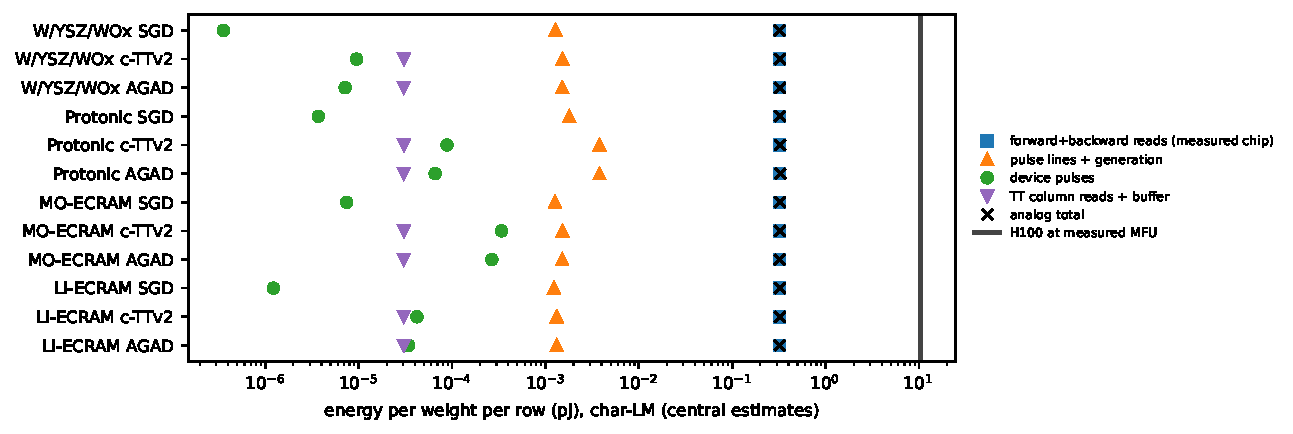
\includegraphics[width=\linewidth]{figs/fig_energy}
\caption{Energy per weight per row on the character LM: the H100 at its measured utilisation against the analog arrays, by
component (central estimates; log axis).}\label{fig:energy}
\end{figure}
